% The dvipsnames option is passed to the xcolor package, which beamer loads
\documentclass[xcolor={dvipsnames}]{beamer}

\usepackage{smpa2152-style}

\title[Political Polling]{Political Polling -- Part II: \\ Practice of Polling}
\author[SMPA 2152]{Data Analysis for Journalism and Political Communication (Fall 2025)}
\date{Prof. Bell}

\begin{document}

%%%%%%%%%%%%%%%%%%%%%%%%%%%%%%%%%%%%%%%%%%%%%%%%%%%%%%%%%%%%%%%%%%}
\frame{
\titlepage
}

%%%%%%%%%%%%%%%%%%%%%%%%%%%%%%%%%%%%%%%%%%%%%%%%%%%%%%%%%%%%%%%%%%
\frame{\frametitle{Types of Survey Samples}

\only<1>{
    \centering
    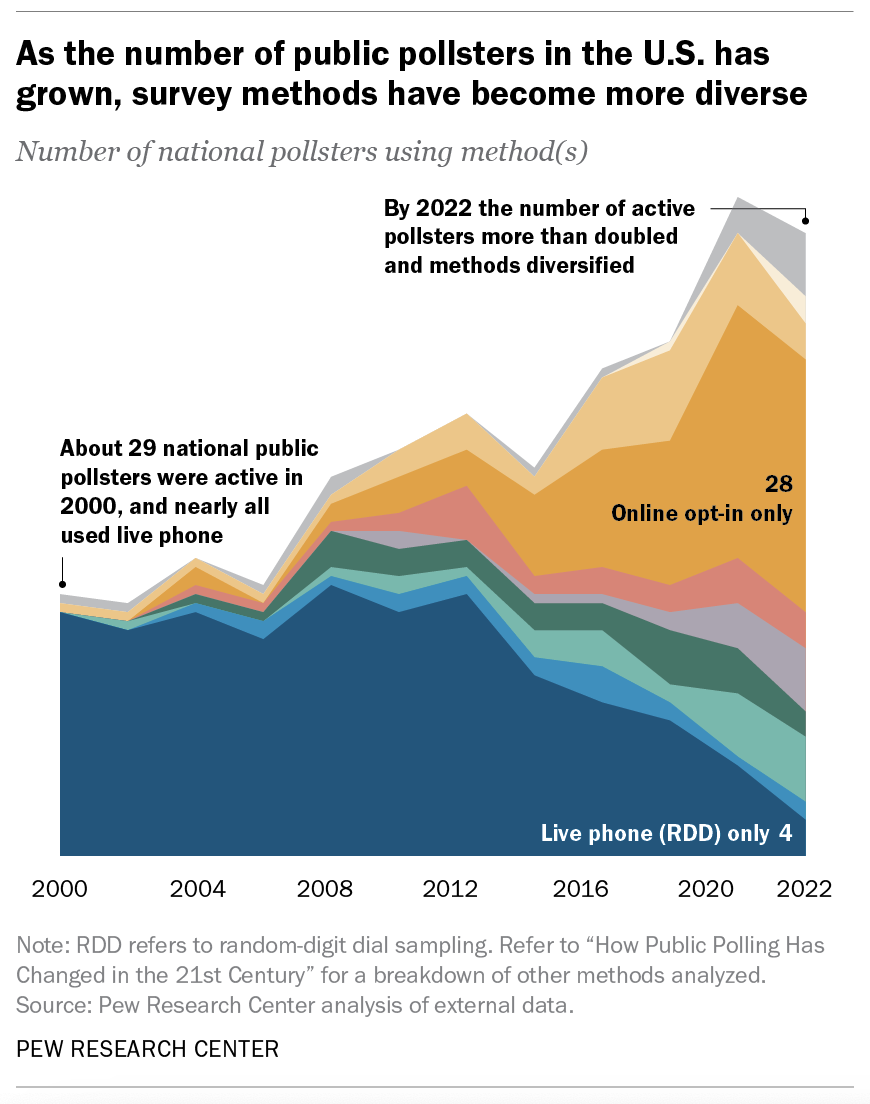
\includegraphics[height = .8\textheight]{survey_types.png}
}

\only<2-4,6-7>{
    \begin{itemize}[<+(1)->]
        \item \textbf{Systematic Sampling}: Select every $n^{th}$ unit of a population (e.g. exit polls)
        \item \textbf{List-based Sampling}: Randomly select units from an existing list of the population (e.g. registered voter lists)
        \item \textbf{Address-based Sampling (ABS)}: Randomly select households from a list of addresses provided by the U.S. Postal Service
        \item<6-> \textbf{Random-digit Dialing (RDD)}: Randomly select area codes, and then random digits are added to the end to create 10-digit phone numbers
        \item<7-> \textbf{Non-probability/Quota Sampling}: Pseudo-randomly selecting, from an opt-in pool of respondents, a sample that approximates the make-up of the general population
    \end{itemize}
}
\only<5>{
    \centering
    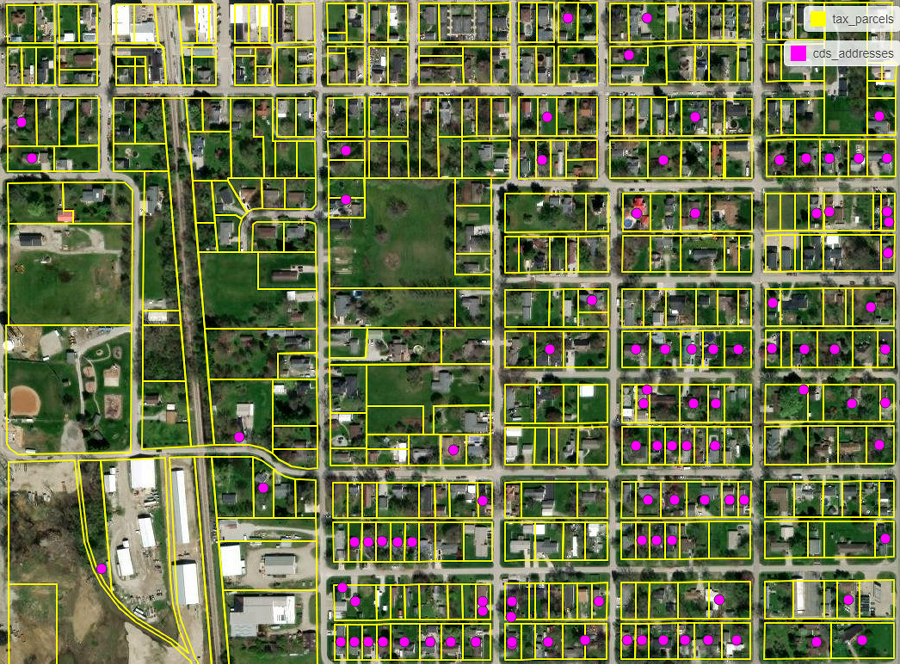
\includegraphics[height = .8\textheight]{norc_gis.png}
}
\only<8>{
    \centering
    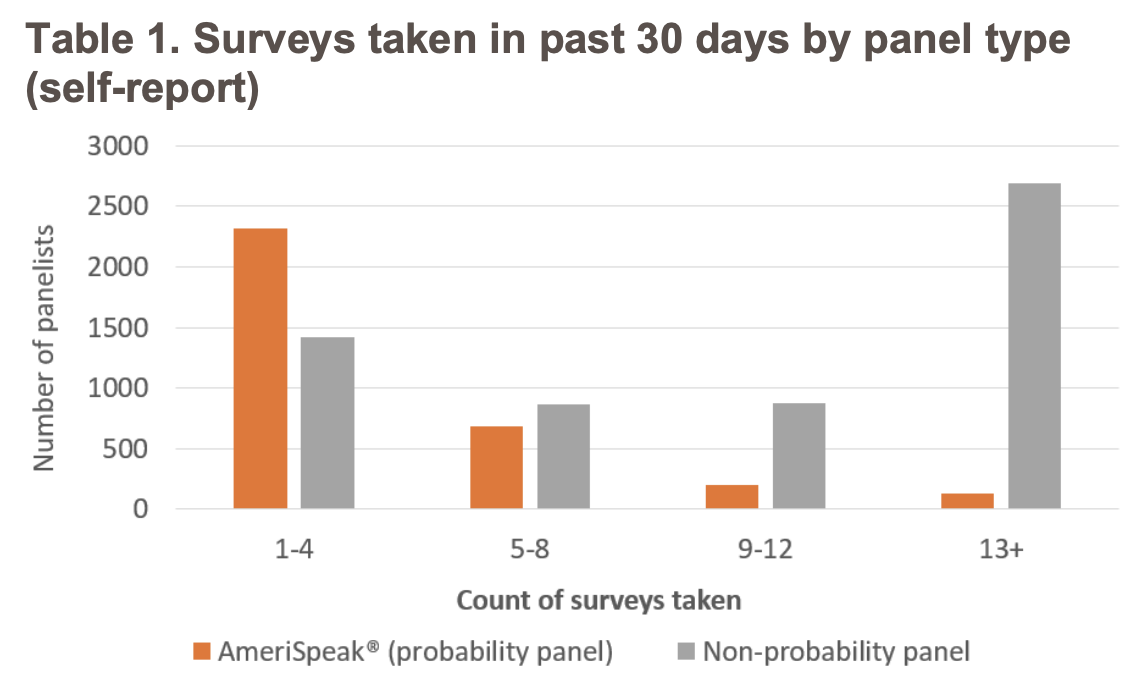
\includegraphics[height = .8\textheight]{norc_professional_respondents.png}
}

}

%%%%%%%%%%%%%%%%%%%%%%%%%%%%%%%%%%%%%%%%%%%%%%%%%%%%%%%%%%%%%%%%%%
\frame{\frametitle{AI and Surveys}
\only<1-2,4-5>{
    \begin{itemize}[<+->]
        \item AI has been successfully applied in survey research, such as transforming open-ended responses into data or evaluating the quality of survey questions (e.g., AI agents can pre-test surveys)
        \item A nascent area of research is the use of ``synthetic personas'' to imitate different types of survey respondents
        \item<4-> With declining survey response rates making representative samples difficult, it may be a viable tradeoff\\
        ~\\
        \textit{``If you're going to pay for polling data that gets the wrong result, you might as well use AI and save money. While surveying real people seems to be getting less accurate over time, the question is whether AI polling will improve.''} - Reed Albergotti (Semafor)
        \item<5-> However, AI models are still not good at ``out-of-sample'' inference, which means these synthetic personas may not generate good data
    \end{itemize}
}

\only<3>{
    \centering
    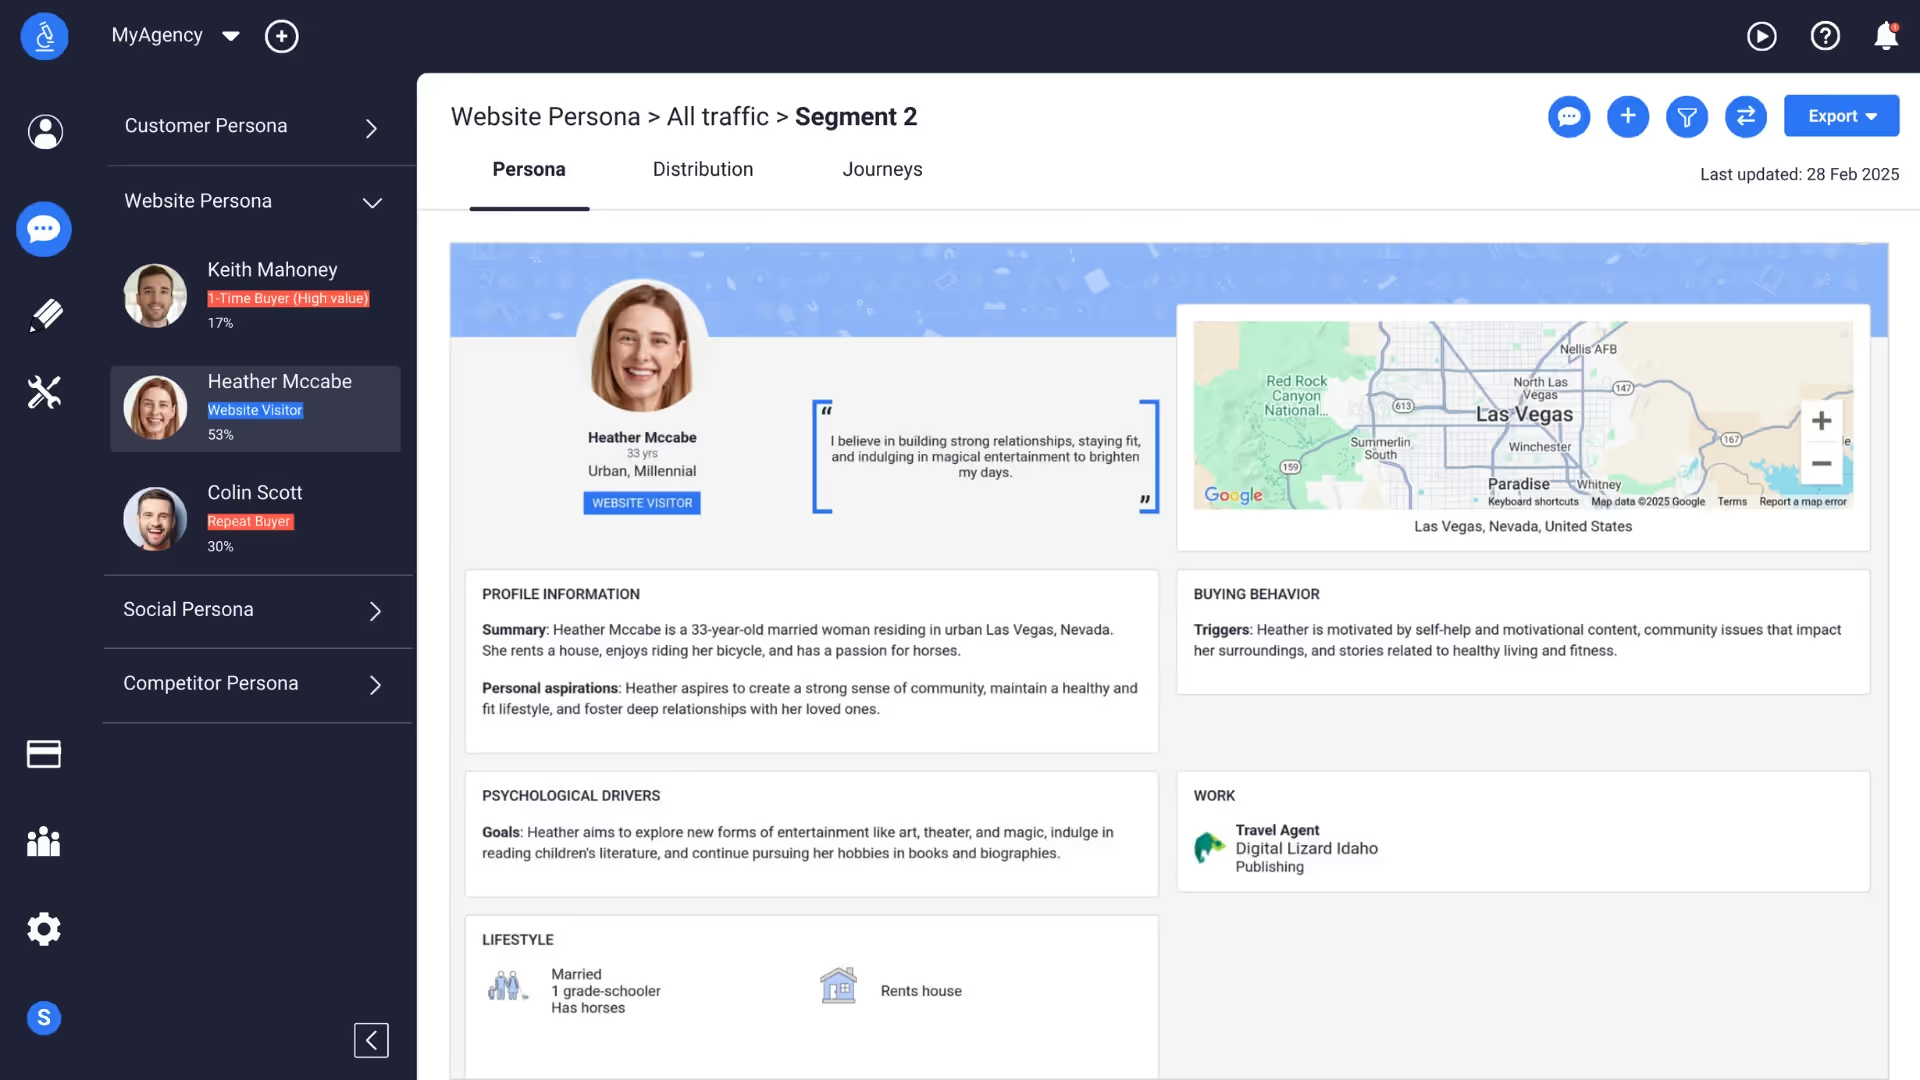
\includegraphics[width = .9\textwidth]{delve_ai_synthetic_persona.png}
}
\only<6>{
    \centering
    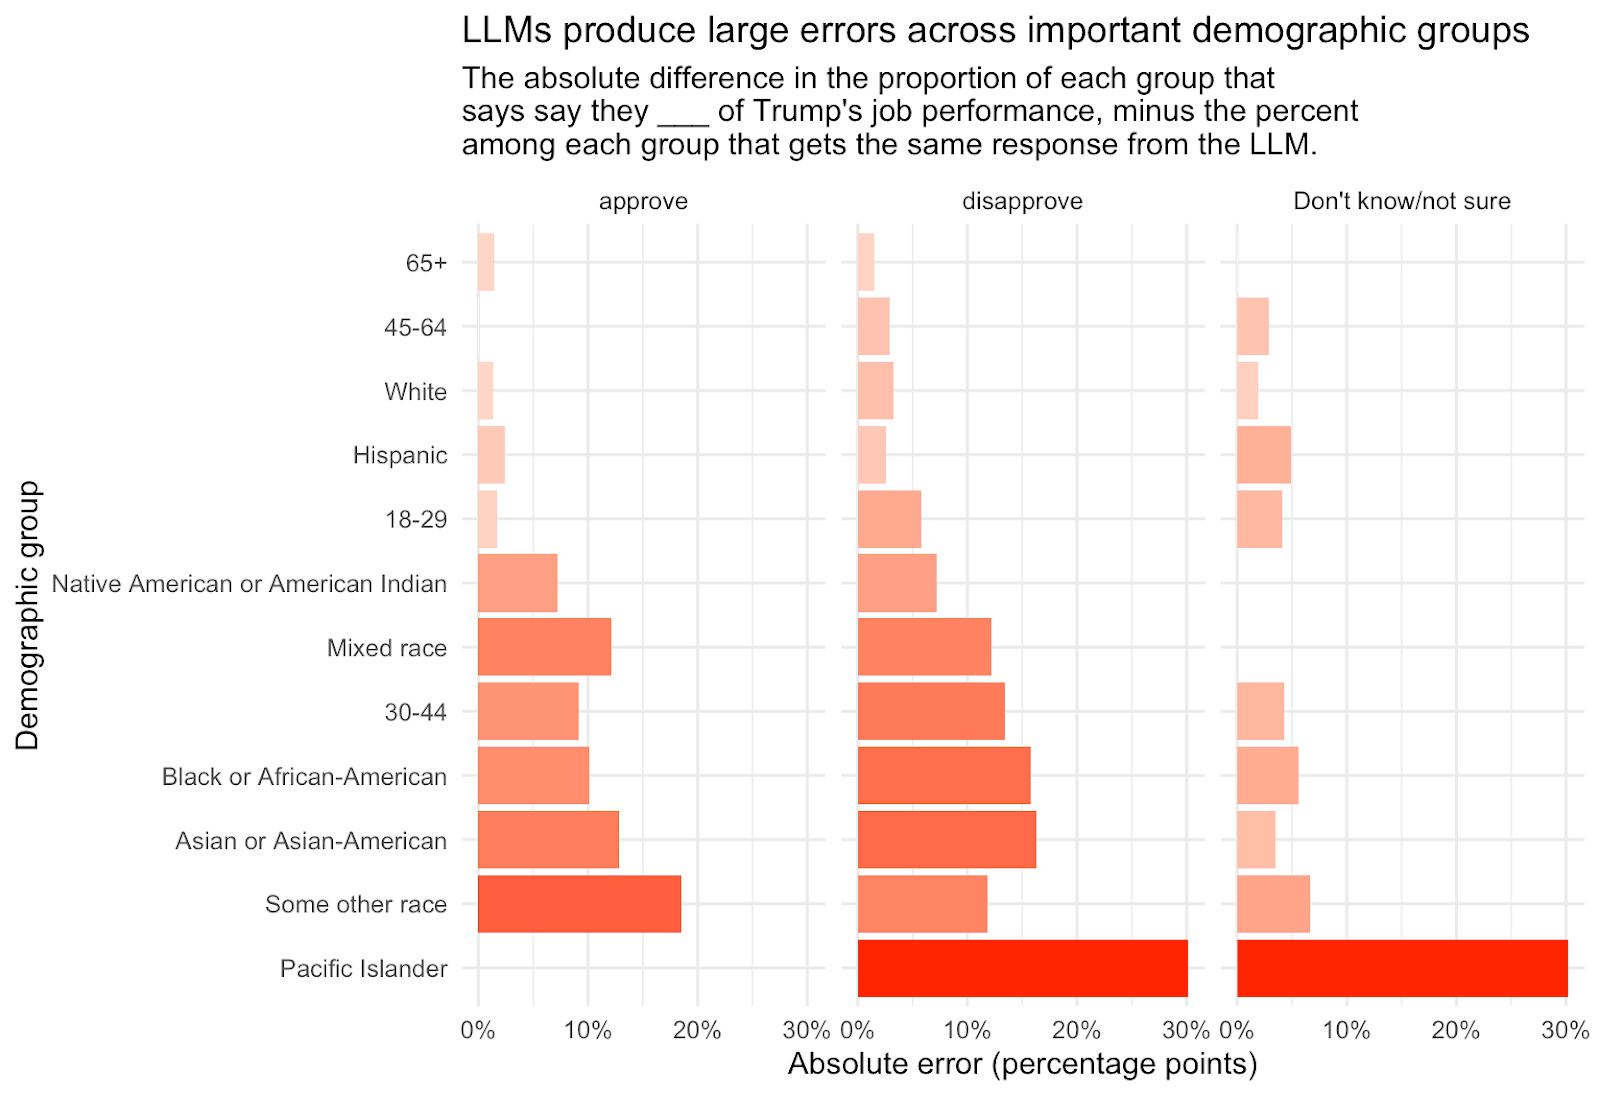
\includegraphics[height = .8\textheight]{llm_survey_errors.png}
}
}

%%%%%%%%%%%%%%%%%%%%%%%%%%%%%%%%%%%%%%%%%%%%%%%%%%%%%%%%%%%%%%%%%%
\frame{\frametitle{Writing Good Surveys}

\only<1-2, 7>{
    \begin{itemize}[<+->]
        \item As with data visualization, we have to assume that we have a limited amount of the respondent's attention
        \item The goal of survey design is to \textit{minimize} cognitive load and \textit{maximize} specificity, but these two goals are often in tension
        \item<7-> When the cognitive load on respondents is too high, they are likely to engage in \textbf{satisficing} or exit the survey entirely (known as survey attrition).
    \end{itemize}
}

\only<3>{
    \centering
    \fbox{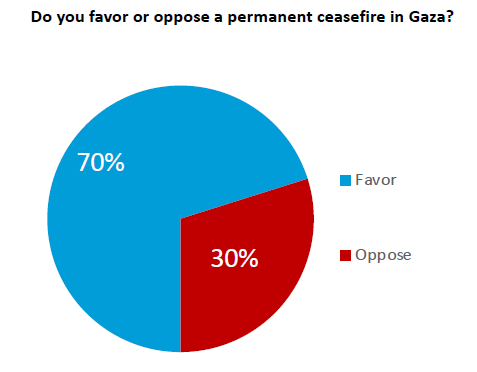
\includegraphics[width = .45\textwidth]{gaza1.png}}
    \fbox{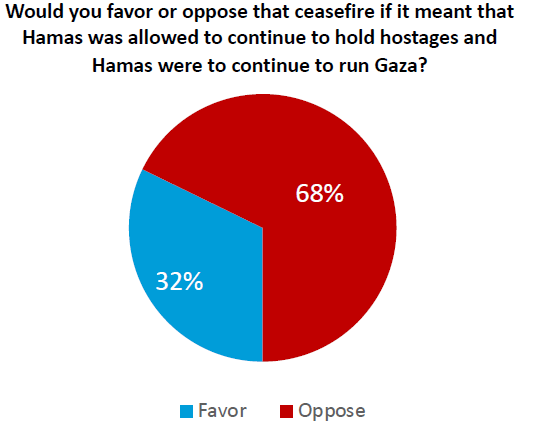
\includegraphics[width = .45\textwidth]{gaza2.png}}
    \\~\\
    \scriptsize Source: Harvard IOP Youth Poll
}

\only<4>{
 \begin{columns}
        \begin{column}{0.5\textwidth}
            \centering
            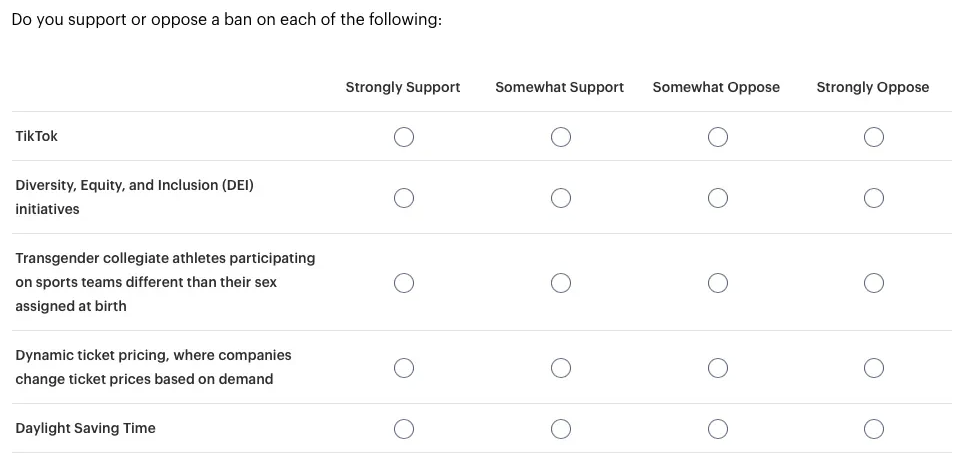
\includegraphics[height=0.25\textheight]{yougov_no_formatting.png}
            ~\\ ~\\
            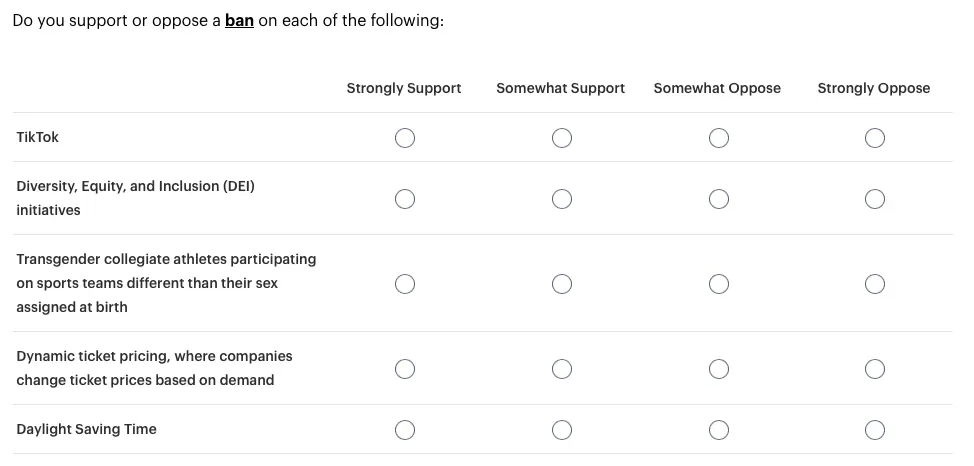
\includegraphics[height=0.25\textheight]{yougov_bold.png}
        \end{column}
        \begin{column}{0.5\textwidth}
        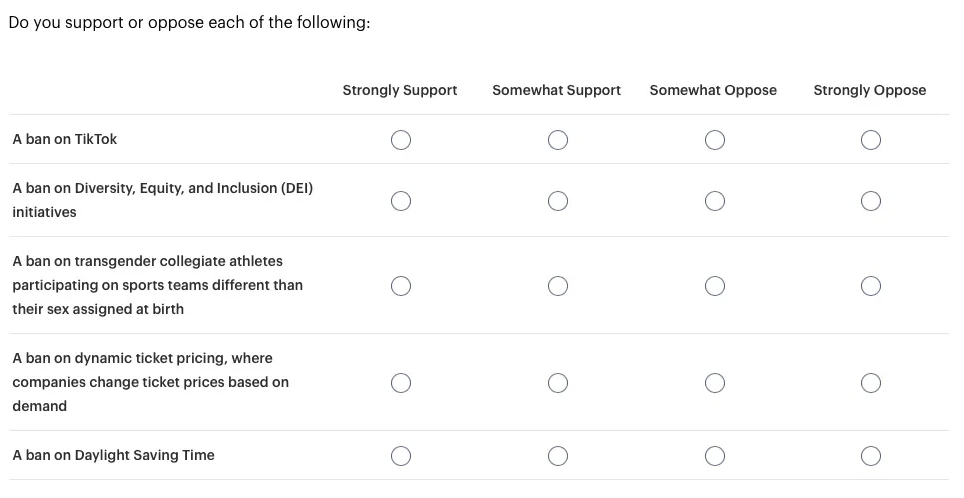
\includegraphics[width=\columnwidth]{yougov_inline.png}
        \end{column}
    \end{columns}
}
\only<5>{
    \centering
    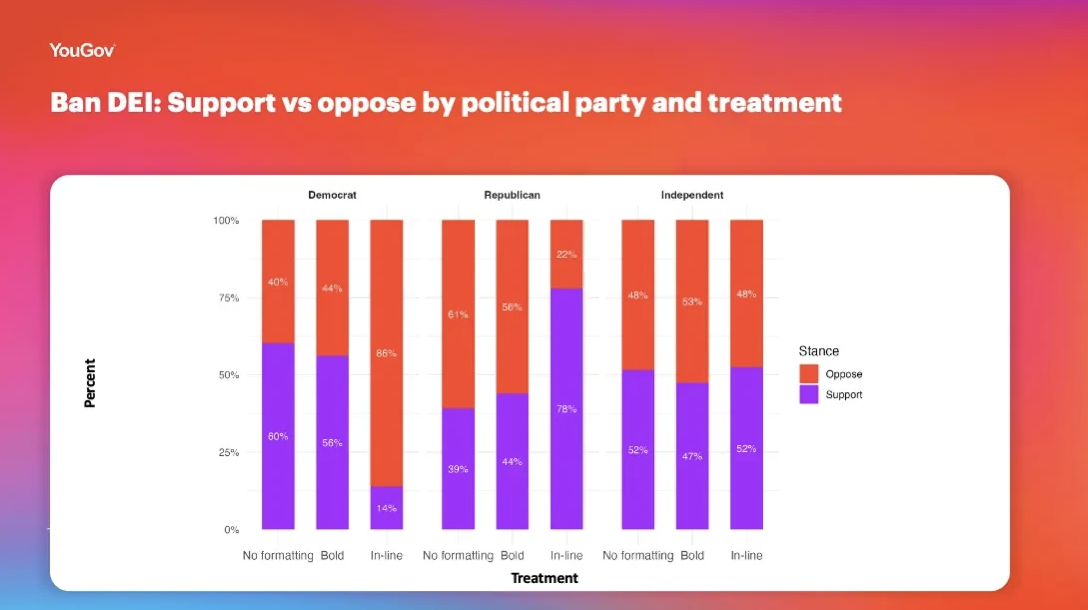
\includegraphics[width = .9\textwidth]{yougov_ban_dei.png}
}
\only<6>{
    \centering
    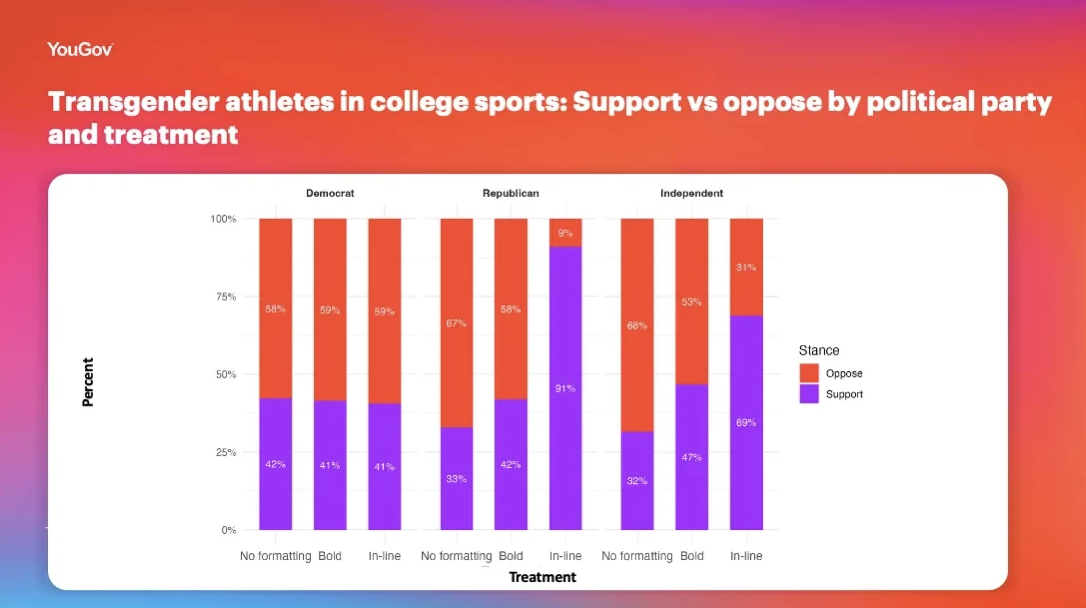
\includegraphics[width = .9\textwidth]{yougov_trans_athletes.png}
}
}

%%%%%%%%%%%%%%%%%%%%%%%%%%%%%%%%%%%%%%%%%%%%%%%%%%%%%%%%%%%%%%%%%%
\frame{\frametitle{Writing Good Surveys}
\only<1-6>{\begin{block}{Satisficing}
Occurs when respondents do not expend the mental effort necessary to generate optimal answers to survey questions
\end{block}
~\\
\only<2-6>{Jon Krosnick (1991) identifies several types of satisficing:
\begin{enumerate}[<+(1)->]
    \item Picking the first or last answer
    \item Agreeing/acquiescing
    \item ``Straight-lining''
    \item Saying ``don't know''
    \item Mental coin-flipping
\end{enumerate}
}}
\only<7>{
    \centering
    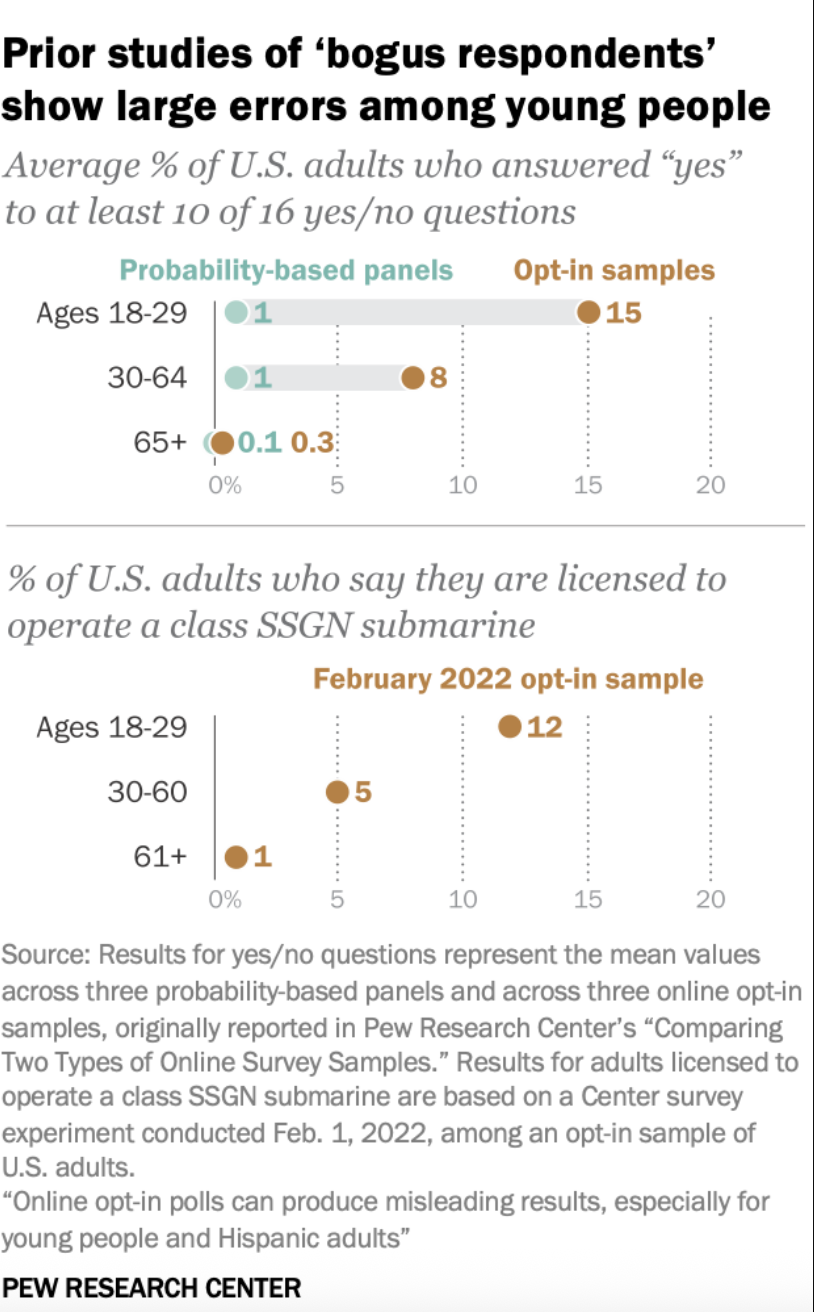
\includegraphics[height = .8\textheight]{pew_opt_in_young_people.png}
}
}

%%%%%%%%%%%%%%%%%%%%%%%%%%%%%%%%%%%%%%%%%%%%%%%%%%%%%%%%%%%%%%%%%%
\frame{\frametitle{How Can We Avoid Satisficing?}

\only<1>{
    \href{https://www.youtube.com/watch?v=eFzGdQrr2K8}{Methods 101: Question Wording (Pew Research Center)}
}

\only<2-9>{
    \begin{enumerate}[<+(1)->]
        \item Keep question and survey length to a minimum
        \item Put high-cognition questions earlier in the survey, and low-cognition questions (like demographics) at the end of the survey
        \item Use simple, unambiguous language
        \item Avoid leading questions or putting questions in an order that ``primes'' the respondent to think a particular way
        \item Avoid double-barreled questions (``To what extent do you agree with the Biden Administration's plan to forgive \$20,000 of student loans for Pell Grant recipients and \$10,000 of student loans for most other borrowers?'')
        \item Use a concise, mutually-exclusive, and complete set of response options (e.g., Likert scale)
        \item Use open-ended questions judiciously
        \item Pre-test your survey
    \end{enumerate}
}

\only<10>{
    \centering
    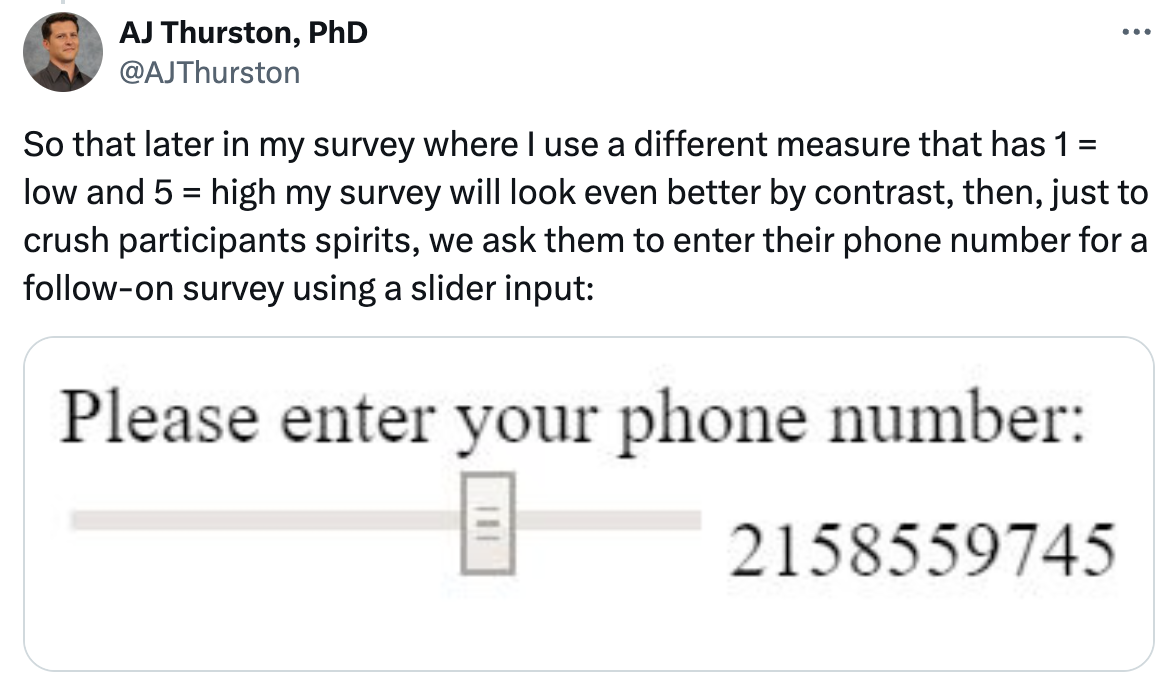
\includegraphics[width = .8\textwidth]{survey_chaos.png}
}
}

%%%%%%%%%%%%%%%%%%%%%%%%%%%%%%%%%%%%%%%%%%%%%%%%%%%%%%%%%%%%%%%%%%
\frame{\frametitle{Finding Polling Data}

\Large
\href{https://ropercenter.cornell.edu/ipoll/}{Link to Roper iPoll}
}

%%%%%%%%%%%%%%%%%%%%%%%%%%%%%%%%%%%%%%%%%%%%%%%%%%%%%%%%%%%%%%%%%%
\frame{\frametitle{In-Class Exercise}

\begin{enumerate}
    \item Search for a topic that you are interested in and select a question
    \item Calculate the margin of error for the response options of interest (i.e., ignore ``don't know''). Are you confident that there is a difference between these proportions?
    \begin{itemize}
        \item Recall the formula for margin of error from last week: $1.96 * \sqrt{(p * (1 - p)) / n}$
    \end{itemize}
    \item Evaluate the question wording. Is this a well-written survey question? Why or why not?
\end{enumerate}
}

\end{document}
